\chapter{Descripción del proyecto}

\section{Visión general de OmniLitter}

OmniLitter es una plataforma multiplataforma desarrollada con el objetivo de facilitar la monitorización y el análisis de residuos en distintos tipos de entornos: playas, riberas, bosques y zonas urbanas. El sistema está orientado tanto a investigadores como a colaboradores de campo, proporcionando herramientas que permiten registrar, almacenar y analizar información relacionada con campañas de muestreo de residuos.

La finalidad de la plataforma no es únicamente contabilizar residuos, sino digitalizar y unificar la toma de datos para que las observaciones puedan convertirse en información científica comparable. Para ello, OmniLitter organiza el trabajo en campañas y sesiones de muestreo, registra metadatos de campo, utiliza categorías estandarizadas de residuos y conserva la localización y evidencias asociadas a cada observación.

La arquitectura de OmniLitter se compone de tres elementos principales estrechamente
integrados: una API central, una aplicación móvil y un portal web. La aplicación
móvil se orienta a la recogida de datos en campo, el portal web a la gestión y
explotación de la información, y la API actúa como punto común de autenticación,
validación, persistencia y sincronización.

Esta aproximación permite conectar la recogida de datos con la evaluación de tendencias y medidas de mitigación. Al conservar datos cuantitativos, metadatos y trazabilidad por campaña, la plataforma puede apoyar comparaciones antes y después de una intervención, ayudar a identificar fuentes probables de contaminación y aportar evidencias para valorar la eficacia de políticas o acciones de reducción de residuos.

\section{Actores y perfiles de usuario}

OmniLitter es una plataforma colaborativa en la que distintos usuarios participan en la gestión de campañas de monitorización y en la recogida de observaciones de residuos. Debido a esta naturaleza colaborativa, el sistema implementa un modelo de control de acceso basado en dos conceptos diferenciados: el rol global del usuario dentro de la plataforma y el rol que dicho usuario posee dentro de cada grupo de trabajo.

Esta separación permite que una misma persona pueda desempeñar diferentes responsabilidades según el grupo en el que participe, garantizando al mismo tiempo el aislamiento de la información entre equipos de trabajo independientes.

El acceso a los datos se estructura alrededor de tres elementos fundamentales:

\begin{itemize}
    \item La cuenta de usuario, que identifica a la persona dentro de la plataforma.
    \item El grupo de trabajo, que delimita el conjunto de campañas, sesiones y observaciones accesibles.
    \item El rol asignado, que determina las acciones que el usuario puede realizar sobre dichos datos.
\end{itemize}

\begin{figure}[H]
\centering
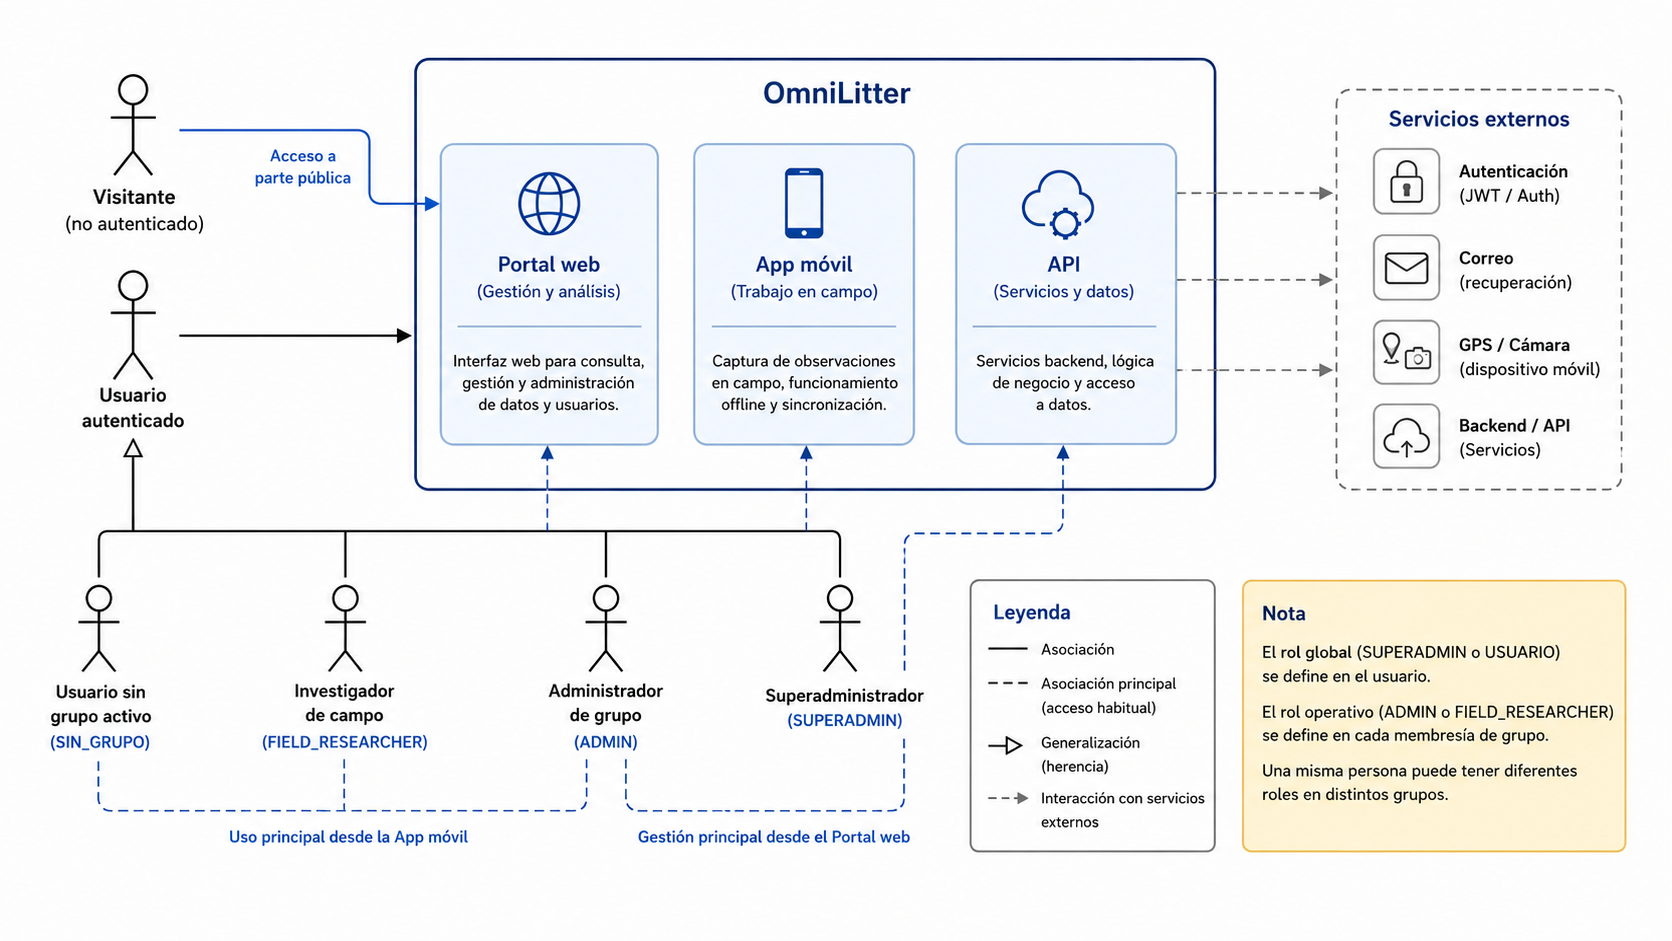
\includegraphics[width=0.92\textwidth]{figures/actores_perfiles.png}
\caption{Actores y perfiles de usuario contemplados en OmniLitter.}
\label{fig:actores_perfiles}
\end{figure}

A continuación se describen los principales perfiles contemplados por el sistema.

\subsection{Visitante}

El visitante corresponde a cualquier persona que accede a la parte pública de la plataforma sin haber iniciado sesión. Este perfil únicamente puede consultar información general sobre OmniLitter y acceder a las funcionalidades de autenticación, como el inicio de sesión, el registro de una nueva cuenta o la recuperación de contraseña.

No dispone de acceso a campañas, observaciones, métricas ni información perteneciente a los grupos de trabajo.

\subsection{Usuario autenticado}

El usuario autenticado constituye el perfil base del sistema. Se trata de cualquier persona que dispone de una cuenta válida y ha iniciado sesión correctamente.

Este perfil puede gestionar la información asociada a su propia cuenta, consultar los grupos a los que pertenece, seleccionar un grupo activo y aceptar o rechazar invitaciones recibidas. Sin embargo, los permisos operativos sobre campañas y observaciones dependen del rol que posea dentro de cada grupo.

\subsection{Investigador de campo}

El investigador de campo es el perfil responsable de la recogida de información durante las campañas de monitorización. Su actividad principal se desarrolla mediante la aplicación móvil, desde la cual puede crear sesiones de muestreo, registrar observaciones, clasificar residuos mediante la taxonomía disponible, adjuntar fotografías y capturar la localización geográfica de cada registro.

Además, este perfil puede trabajar en modo offline cuando no existe conectividad, almacenando localmente la información para sincronizarla posteriormente con el servidor.

Aunque puede consultar la información necesaria para desarrollar su trabajo, no dispone de permisos para administrar usuarios, gestionar campañas o modificar la estructura organizativa del grupo.

\subsection{Administrador de grupo}

El administrador de grupo es el responsable de coordinar la actividad de un grupo de trabajo concreto. Este perfil puede gestionar los miembros del grupo, enviar invitaciones, asignar roles de membresía y administrar las campañas asociadas a dicho grupo.

Entre sus funciones se encuentran la creación, edición y organización de campañas de monitorización, así como la supervisión de la actividad realizada por los investigadores de campo. También dispone de acceso a métricas agregadas e información de seguimiento relacionada con las campañas del grupo.

Sus permisos se limitan exclusivamente a los grupos en los que posee dicho rol. Por tanto, un mismo usuario puede actuar como administrador en un grupo y como investigador de campo en otro diferente.

\subsection{Superadministrador}

El superadministrador representa el perfil con mayor nivel de autoridad dentro de OmniLitter. Su función principal consiste en administrar la plataforma a nivel global y garantizar su correcto funcionamiento.

Este perfil puede gestionar usuarios, modificar roles globales, supervisar grupos de trabajo y realizar tareas de soporte operativo dentro de la plataforma. A diferencia del administrador de grupo, sus permisos no se encuentran restringidos a un único grupo, sino que abarcan la totalidad del sistema.

Debido a su alcance, este perfil está destinado a tareas de administración y soporte de la plataforma, y no a la realización de actividades habituales de monitorización en campo.

\subsection{Usuario sin grupo activo}

Finalmente, OmniLitter contempla la situación de usuarios registrados que todavía no pertenecen a ningún grupo o que no han seleccionado uno como grupo activo.

En este estado, el usuario puede gestionar su cuenta personal y revisar invitaciones pendientes, pero no tiene acceso a campañas, observaciones ni funcionalidades relacionadas con la monitorización hasta incorporarse a un grupo de trabajo.

\subsection{Actores de apoyo}

Además de los usuarios que interactúan directamente con la plataforma, OmniLitter depende de diversos componentes técnicos que permiten el funcionamiento del sistema.

Entre ellos destacan el servicio de autenticación encargado de validar credenciales y gestionar sesiones, el servicio de correo utilizado para determinadas comunicaciones automáticas, los dispositivos móviles empleados durante las campañas de campo y la infraestructura backend responsable de la lógica de negocio y el almacenamiento persistente de la información.

Aunque estos elementos no representan usuarios propiamente dichos, constituyen actores fundamentales para la correcta ejecución de los procesos definidos por la plataforma.

\section{Plataformas del sistema}

OmniLitter se concibe como una plataforma compuesta por varios elementos que colaboran entre sí para cubrir las distintas fases del proceso de monitorización de residuos. La naturaleza del problema exige disponer de herramientas adaptadas tanto al trabajo de campo como a la gestión y análisis posterior de la información recopilada.

Para dar respuesta a estas necesidades, el sistema se estructura en tres componentes principales: una aplicación móvil, un portal web y un backend centralizado. Esta separación permite adaptar cada componente a las tareas específicas que debe desempeñar, manteniendo al mismo tiempo una gestión unificada de la información.

\begin{figure}[H]
\centering
\begin{subfigure}{0.86\textwidth}
    \centering
    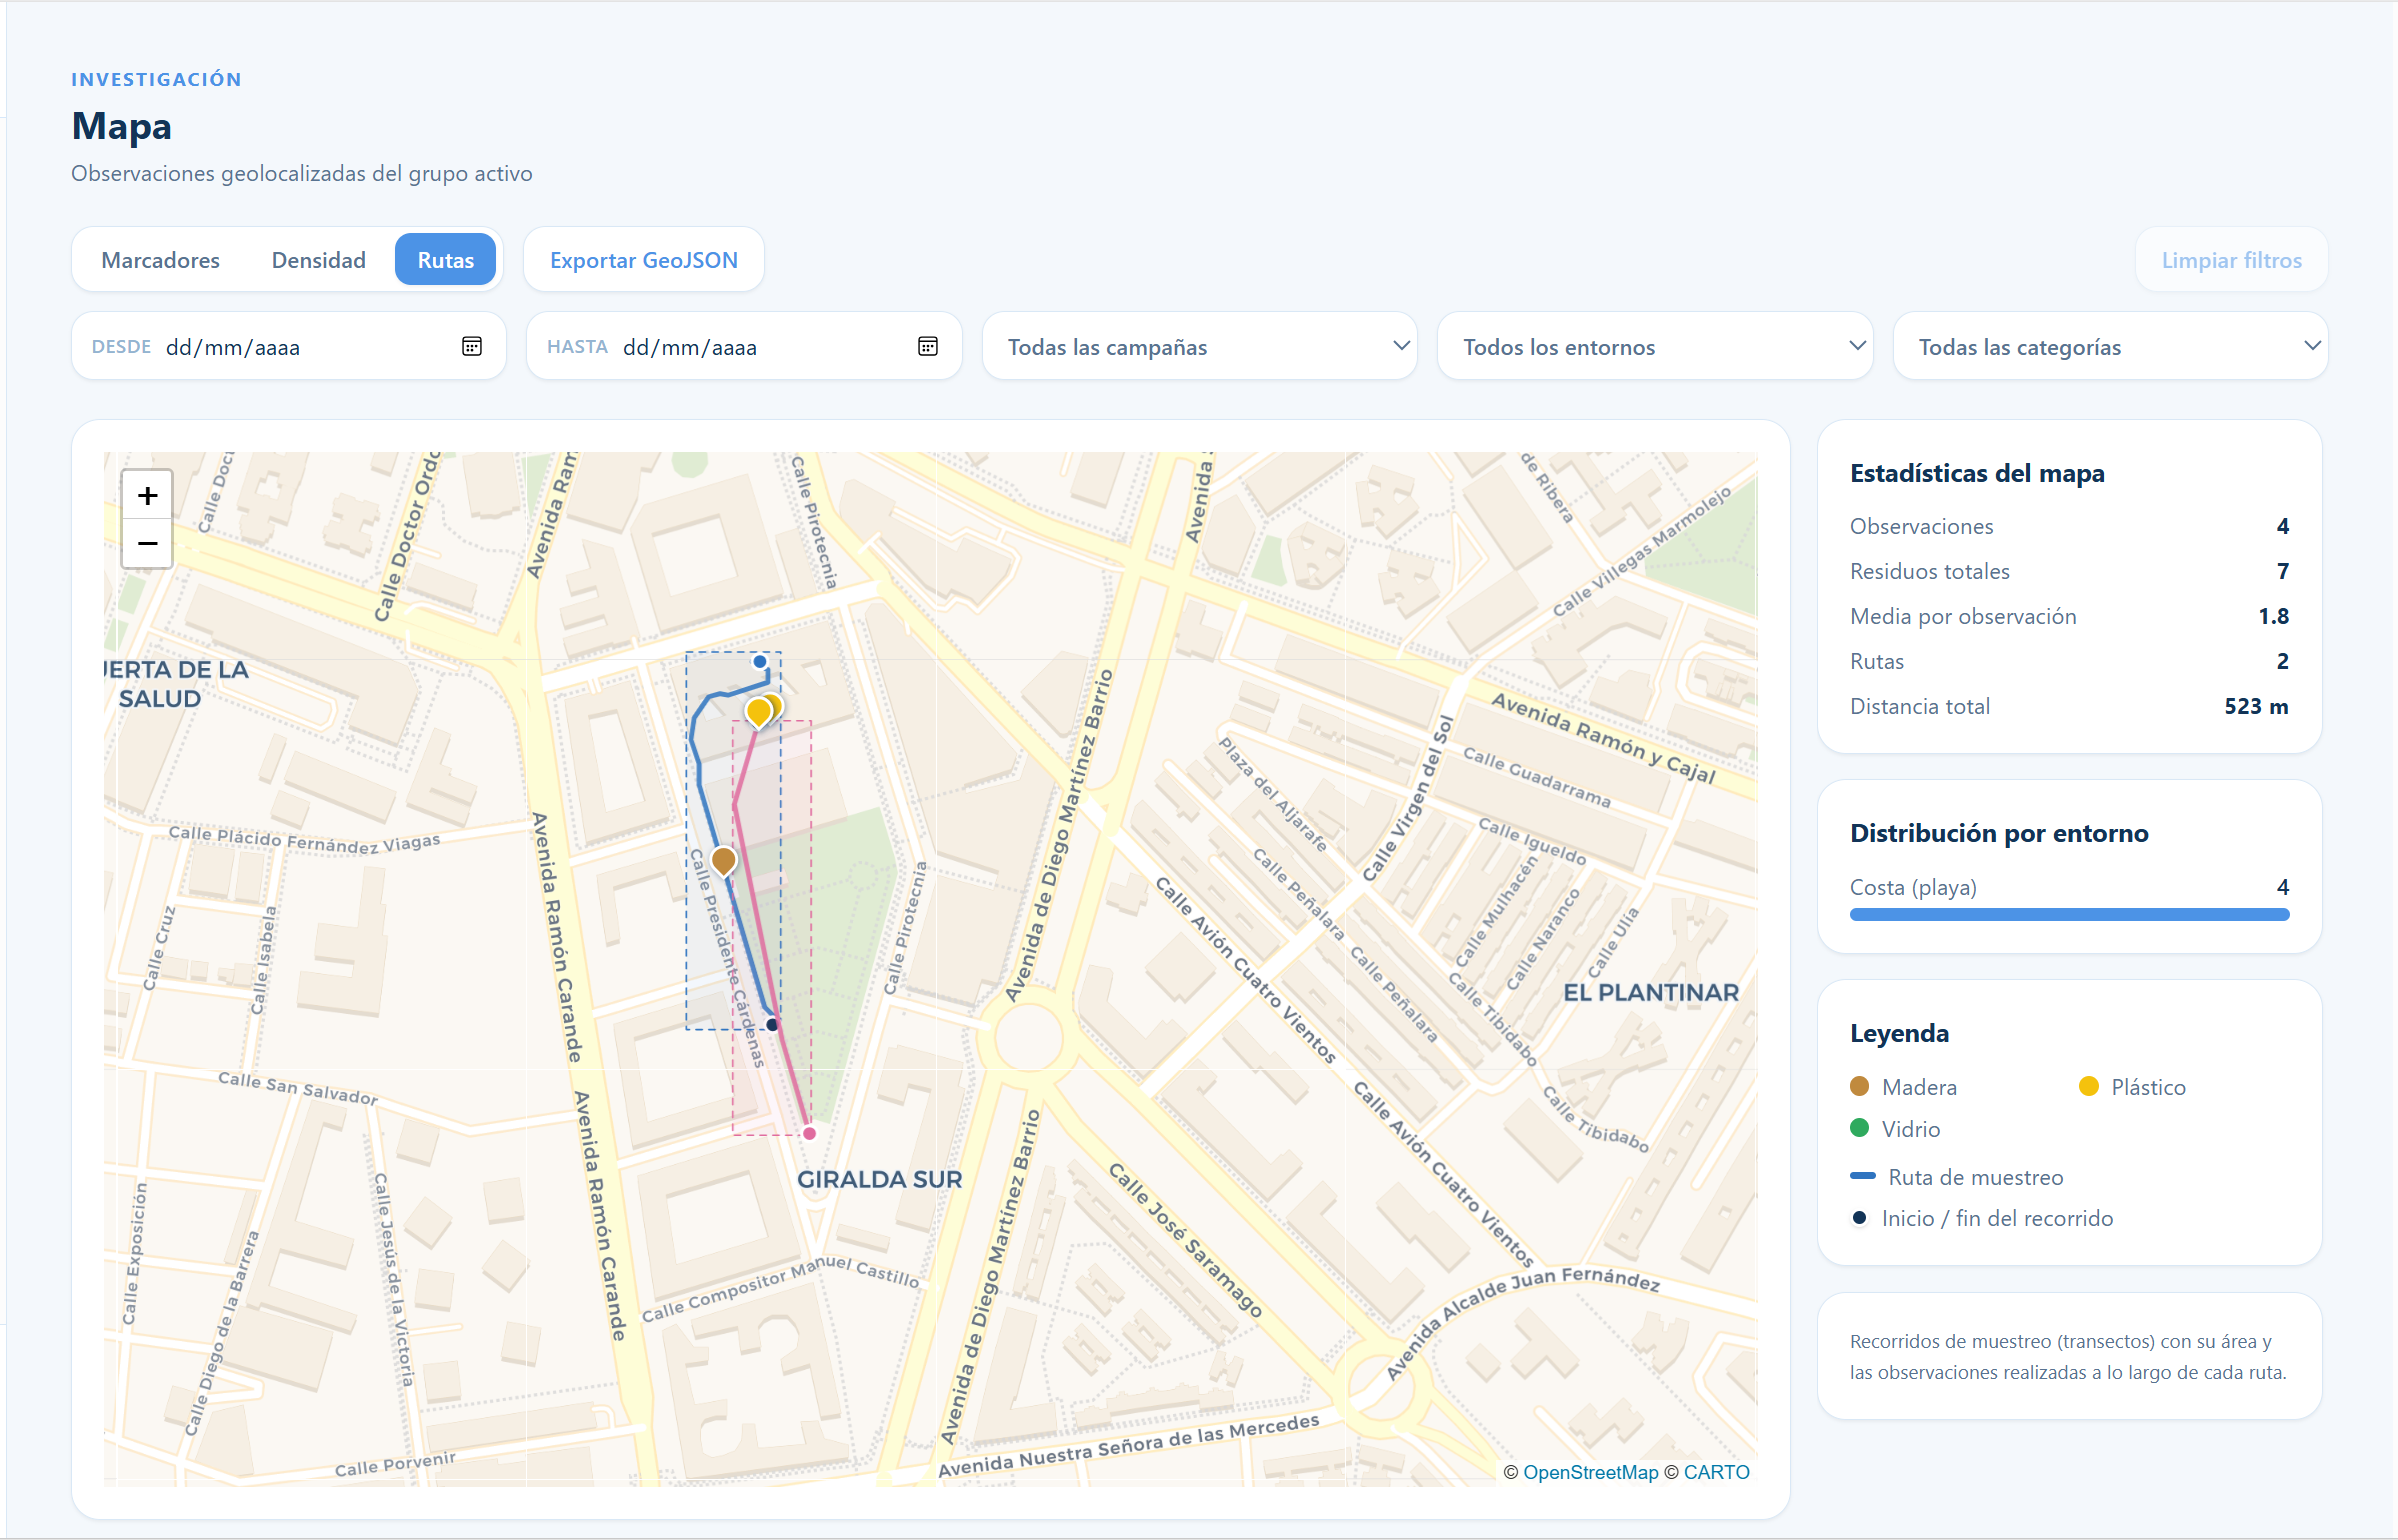
\includegraphics[width=\textwidth]{figures/mapa-web.png}
    \caption{Portal web para la consulta geográfica de observaciones.}
\end{subfigure}

\vspace{0.45em}

\begin{subfigure}{0.30\textwidth}
    \centering
    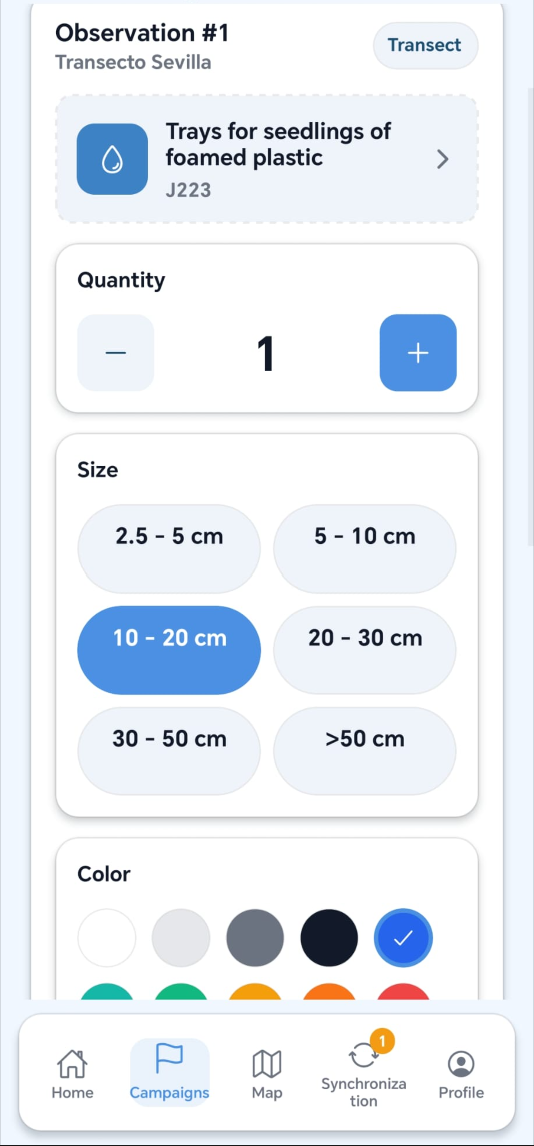
\includegraphics[width=\textwidth]{figures/creacion-observacion-movil.png}
    \caption{Aplicación móvil para el registro de observaciones en campo.}
\end{subfigure}
\caption{Vista general de las dos plataformas principales utilizadas por OmniLitter.}
\label{fig:vista_producto_web_movil}
\end{figure}

\subsection{Aplicación móvil}

La aplicación móvil constituye la herramienta principal para la recogida de datos en campo. Está orientada a los usuarios que participan directamente en las campañas de monitorización y les permite registrar observaciones de residuos en el lugar donde se producen.

A través de esta aplicación es posible consultar campañas, iniciar sesiones de muestreo, registrar observaciones, capturar fotografías asociadas a los residuos encontrados y almacenar la localización geográfica de cada registro. Además, la aplicación está diseñada para funcionar en entornos con conectividad limitada, permitiendo continuar el trabajo incluso cuando no existe acceso a Internet y sincronizando posteriormente la información con el servidor.

\subsection{Portal web}

El portal web proporciona las herramientas necesarias para la gestión y supervisión de la información recopilada. Esta plataforma está orientada principalmente a administradores de grupo, investigadores y superadministradores.

Desde el portal web es posible gestionar usuarios y grupos de trabajo, crear y administrar campañas de monitorización, consultar observaciones registradas, visualizar información geográfica mediante mapas interactivos y acceder a métricas agregadas sobre los datos recopilados. Asimismo, permite exportar la información para su utilización en procesos posteriores de análisis científico.

A diferencia de la aplicación móvil, cuyo objetivo principal es facilitar la recogida de datos en campo, el portal web está enfocado a la coordinación, revisión y explotación de la información almacenada.

\subsection{Backend y almacenamiento centralizado}

El backend actúa como elemento de coordinación entre las distintas plataformas del sistema. Su función consiste en centralizar la lógica de negocio, gestionar la autenticación de usuarios, controlar los permisos de acceso y garantizar la consistencia de los datos almacenados.

Tanto la aplicación móvil como el portal web se comunican con este componente para consultar o registrar información. De esta forma, todas las operaciones se realizan sobre una única fuente de datos común, evitando inconsistencias y facilitando la gestión centralizada del sistema.

La información recopilada durante las campañas se almacena en una base de datos centralizada que actúa como repositorio principal de usuarios, grupos, campañas, sesiones de muestreo, observaciones y fotografías asociadas.

\subsection{Integración de las plataformas}

La combinación de estas plataformas permite cubrir el ciclo completo de trabajo de una campaña de monitorización. La aplicación móvil facilita la recogida de datos sobre el terreno, el backend garantiza la gestión y consistencia de la información, y el portal web proporciona las herramientas necesarias para su consulta, supervisión y análisis posterior.

Esta arquitectura permite que cada componente se especialice en una función concreta, favoreciendo la mantenibilidad del sistema y facilitando su evolución futura.


\section{Funcionalidades principales}

OmniLitter proporciona un conjunto de funcionalidades orientadas a cubrir el ciclo completo de una campaña de monitorización de residuos, desde la organización de los equipos de trabajo hasta la recogida y posterior consulta de los datos obtenidos.

\subsection{Gestión de usuarios y grupos}

La plataforma permite el registro y autenticación de usuarios, así como la organización de estos en grupos de trabajo independientes. Cada grupo dispone de sus propias campañas, sesiones y observaciones, garantizando el aislamiento de la información entre equipos.

Además, el sistema incorpora distintos niveles de permisos que permiten diferenciar entre usuarios de campo, administradores de grupo y administradores globales de la plataforma.

\subsection{Gestión de campañas}

OmniLitter permite crear y administrar campañas de monitorización asociadas a un grupo de trabajo. Cada campaña define el contexto en el que se desarrollarán las actividades de muestreo, incluyendo información descriptiva, fechas de realización y características generales del entorno estudiado.

Las campañas actúan como elemento organizador de toda la información recogida durante el trabajo de campo.

\subsection{Sesiones de muestreo}

Dentro de cada campaña, los usuarios pueden crear sesiones de muestreo que representan actividades concretas de recogida de datos.

Las sesiones permiten registrar información contextual relacionada con el trabajo realizado, como el entorno de estudio, el método de muestreo empleado, el protocolo aplicado, la duración de la actividad, el tipo de transecto o cuadrante y la ubicación geográfica asociada.

Esta funcionalidad aporta trazabilidad a los datos recopilados, permitiendo conocer las condiciones bajo las que se registró cada observación.

\subsection{Registro de observaciones}

El registro de observaciones constituye la funcionalidad principal del sistema. Durante una sesión de muestreo, los usuarios pueden documentar los residuos encontrados indicando su localización, fecha de registro y clasificación correspondiente.

Cada observación queda vinculada a una campaña y una sesión concretas, permitiendo mantener la coherencia y organización de los datos almacenados.

\subsection{Clasificación mediante taxonomías}

La plataforma incorpora una taxonomía de residuos que permite clasificar las observaciones de forma homogénea y estandarizada, tomando como referencia listas comunes de categorías utilizadas en monitorización de basuras.

El uso de categorías comunes mejora la calidad de los datos recopilados y facilita su comparación entre campañas, grupos de trabajo, entornos y periodos temporales diferentes.

\subsection{Registro fotográfico y geolocalización}

Las observaciones pueden complementarse mediante fotografías y coordenadas geográficas obtenidas desde el dispositivo móvil.

Estas evidencias permiten contextualizar cada registro, aumentar la fiabilidad de los datos y facilitar posteriores procesos de revisión y análisis.

\subsection{Trabajo offline y sincronización}

La aplicación móvil ha sido diseñada para utilizarse en entornos donde la conectividad puede ser limitada o inexistente.

Por este motivo, los usuarios pueden continuar registrando observaciones sin conexión a Internet. Cuando la conectividad se restablece, la información almacenada localmente se sincroniza con el sistema central, garantizando la disponibilidad de los datos para el resto de usuarios autorizados.

\subsection{Consulta y visualización de información}

El portal web permite consultar la información recopilada durante las campañas mediante diferentes mecanismos de visualización.

Los usuarios autorizados pueden revisar observaciones, consultar información geográfica a través de mapas interactivos y acceder a métricas generales relacionadas con la actividad de monitorización realizada.

\subsection{Exportación de datos}

OmniLitter incorpora mecanismos para exportar la información recopilada en formatos adecuados para su tratamiento posterior.

Esta funcionalidad facilita la reutilización de los datos en herramientas externas de análisis y favorece su utilización en estudios científicos relacionados con la contaminación por residuos, incluyendo la generación de series temporales, comparaciones espaciales y evaluaciones de medidas de mitigación.

\subsection{Resumen funcional}

De forma resumida, OmniLitter permite:

\begin{itemize}
    \item Gestionar usuarios, grupos y permisos.
    \item Planificar campañas de monitorización.
    \item Realizar sesiones de muestreo en campo.
    \item Registrar observaciones geolocalizadas.
    \item Clasificar residuos mediante una taxonomía estandarizada.
    \item Asociar fotografías y metadatos a las observaciones.
    \item Trabajar sin conexión y sincronizar posteriormente los datos.
    \item Consultar la información recopilada mediante mapas y métricas.
    \item Exportar los datos para su análisis posterior.
\end{itemize}

\section{Restricciones y alcance excluido}

Con el objetivo de acotar el alcance del proyecto y ajustarlo a las limitaciones temporales y de recursos propias de un Trabajo Fin de Grado, se decidió excluir una serie de funcionalidades y actividades que, aunque podrían aportar valor a la plataforma, no resultaban imprescindibles para cumplir los objetivos principales establecidos.

Las principales exclusiones son las siguientes:

\begin{itemize}

    \item \textbf{Soporte multiidioma avanzado.} Aunque la arquitectura de la aplicación permite la internacionalización de la interfaz, el alcance del proyecto se limita al español y al inglés. La incorporación de idiomas adicionales requeriría un esfuerzo significativo de traducción y mantenimiento, además de depender en algunos casos de servicios externos incompatibles con los requisitos de funcionamiento offline de la aplicación móvil.

    \item \textbf{Mantenimiento evolutivo y correctivo posterior a la entrega.} El presente trabajo contempla el análisis, diseño, implementación y validación de la plataforma. Las actividades relacionadas con el mantenimiento posterior, incorporación de nuevas funcionalidades o soporte continuado tras la finalización del proyecto quedan fuera de su alcance.

    \item \textbf{Identificación automática de residuos mediante inteligencia artificial.} Durante las fases iniciales del proyecto se consideró la posibilidad de incorporar mecanismos de reconocimiento automático de residuos a partir de imágenes. Sin embargo, el desarrollo, entrenamiento y validación de modelos de visión artificial requiere una inversión de tiempo, recursos computacionales y conjuntos de datos especializados que exceden las posibilidades de este Trabajo Fin de Grado.

    \item \textbf{Publicación oficial en tiendas de aplicaciones.} Aunque la aplicación móvil ha sido desarrollada para poder ejecutarse en dispositivos reales, la publicación oficial en plataformas como Google Play Store o Apple App Store no forma parte del alcance del proyecto. Este proceso implica requisitos administrativos, costes económicos y procedimientos de revisión que no resultan necesarios para la validación académica de la solución desarrollada.

\end{itemize}

Estas exclusiones permiten concentrar los esfuerzos de desarrollo en las funcionalidades esenciales de OmniLitter, garantizando una solución completa y funcional dentro de las restricciones temporales y organizativas del proyecto.
